% ==============================================================================
% LAB 119
% UNDERSÖKNING AV RC-KRETS
% ------------------------
%
% Author:
% Jonas Sjöberg     <tel12jsg@student.hig.se>
% Oscar Wallberg    <tco13owg@student.hig.se>
%
% License:
% Creative Commons Attribution-NonCommercial-ShareAlike 4.0 International
% See LICENSE.md for full licensing information.
% ==============================================================================

\section{Uppmätning av stegsvaret}\label{step}
% ------------------------------------------------------------------------------
Stegsvaret mäts genom att kretsen matas med en fyrkantsvåg.
% TODO: 

\subsection{Mätresultat}\label{}
% ------------------------------------------------------------------------------
% TODO:


\subsection{Simulering}\label{}
% ------------------------------------------------------------------------------
Kretsen simuleras i \texttt{Qucs} enligt Figur~\ref{fig:step-sim-step} och
Figur~\ref{fig:step-sim-param}.

\begin{figure}[ht]
    \centering
    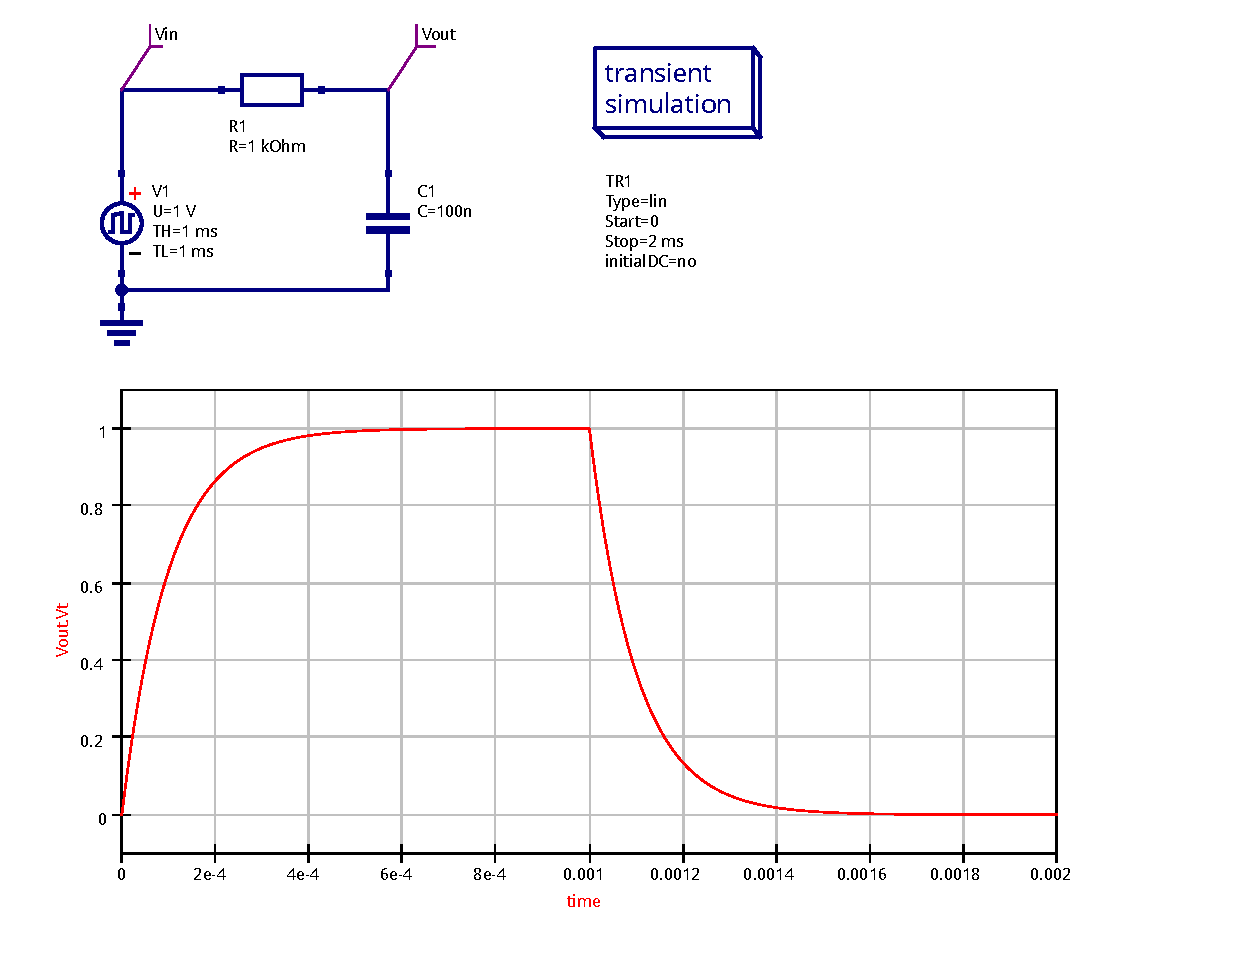
\includegraphics[width=\linewidth]{sim/ee466_lab-4_prj/uppgift-2_step}
    \caption[] {Simulering av kretsens stegsvar.}
    \label{fig:step-sim-step}
\end{figure}

\begin{figure}[ht]
    \centering
    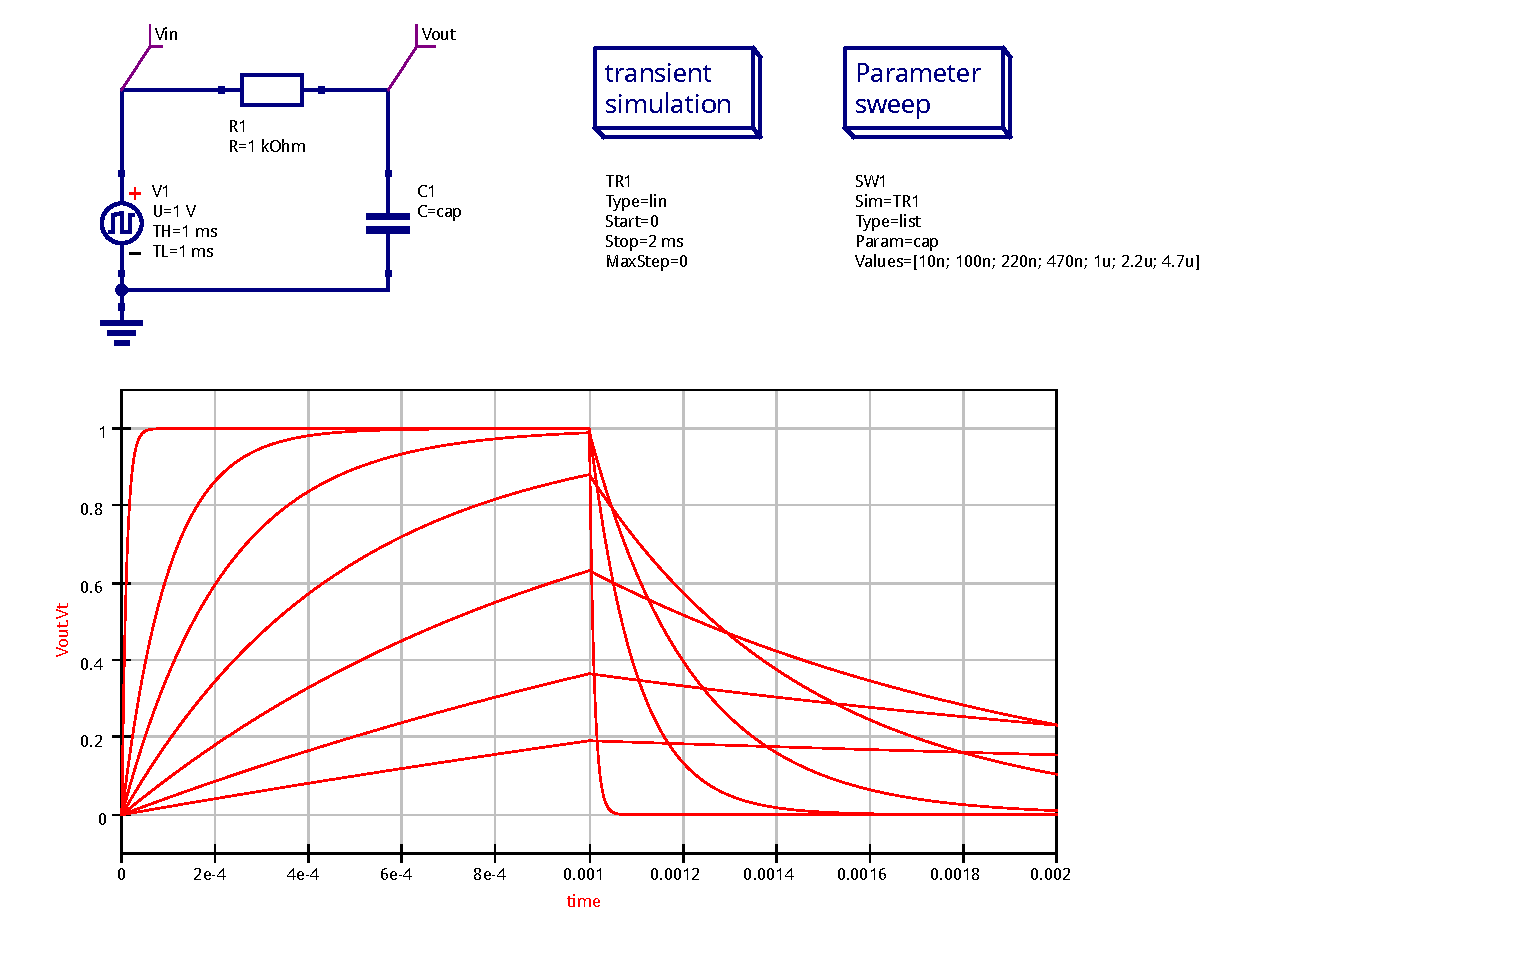
\includegraphics[width=\linewidth]{sim/ee466_lab-4_prj/uppgift-2_param}
    \caption[] {Simulering av kretsens stegsvar för olika värden av $C_1$.}
    \label{fig:step-sim-param}
\end{figure}


\subsection{Kommentar}\label{}
% ------------------------------------------------------------------------------
% TODO:

